\documentclass[11pt,class=report,crop=false]{standalone}
\usepackage[screen]{../python}
\begin{document}



%====================================================================
\chapitre{Dynamic images}
%====================================================================

\objectifs{We will distort images. By repeating these distortions, the images become blurred. But by a miracle after a certain number of repetitions the original image reappears!}

\index{image}

%%%%%%%%%%%%%%%%%%%%%%%%%%%%%%%%%%%%%%%%%%%%%%%%%%%%%%%%%%%%%%%%
%%%%%%%%%%%%%%%%%%%%%%%%%%%%%%%%%%%%%%%%%%%%%%%%%%%%%%%%%%%%%%%%

\begin{cours}[Photo booth transformation]

We start from an $n\times n$ array, with even $n$, each element of the table represents a pixel. The rows are indexed from $i=0$ to $i=n-1$, the columns from $j=0$ to $j=n-1$.
From this image we calculate a new image by moving each pixel according to a transformation, called the \defi{photo booth transformation}.

We cut the original image into small $2\times2$ squares.
Each small square is therefore composed of four pixels. Each of these pixels is sent to four different locations in the new image:
the pixel at the top left remains in an area at the top left, the pixel at the top right of the small square, is sent to an area at the top right of the new image,...

\myfigure{0.7}{
\tikzinput{fig-images-1}
}

For example, the pixel in position $(1,1)$ (symbolized by the letter \mot{D}) is sent to position $(4,4)$.

\medskip

Let's explain this principle through formulas. For each couple $(i,j)$, we calculate its image $(i',j')$ using the photo booth transformation according to the following formulas:
\begin{itemize}
  \item If $i$ and $j$ are even: $(i',j') = (i//2,j//2)$.
  \item If $i$ is even and $j$ is odd: $(i',j') = (i//2,(n+j)//2)$.  
  \item If $i$ is odd and $j$ is even: $(i',j') = ((n+i)//2,j//2)$.
  \item If $i$ and $j$ are odd: $(i',j') = ((n+i)//2,(n+j)//2)$.
\end{itemize}


\medskip

Here is an example of a $4\times 4$ array before (left) and after (right) the photo booth transformation. 
$$\begin{array}{cccc} 
  1& 2& 3& 4\\ 
  5& 6& 7& 8\\  
  9&10&11&12\\  
 13&14&15&16  
\end{array}\qquad\qquad  
\begin{array}{cccc} 
  1& 3& 2& 4\\  
  9&11&10&12\\  
  5& 7& 6& 8\\  
 13&15&14&16
\end{array}$$

Here is a $256 \times 256$ image and its first transformation:

\begin{center}
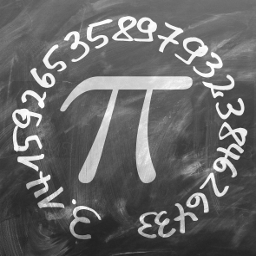
\includegraphics[scale=\myscale,scale=0.4]{images_chapter/pi_gimp_new_photo_0.png}\qquad\qquad
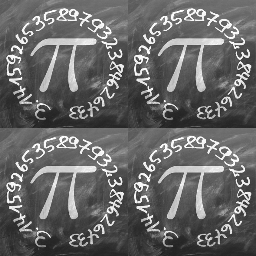
\includegraphics[scale=\myscale,scale=0.4]{images_chapter/pi_gimp_new_photo_1.png}
\end{center}

Here is what happens if you repeat the photo booth transformation several times:
\begin{center}
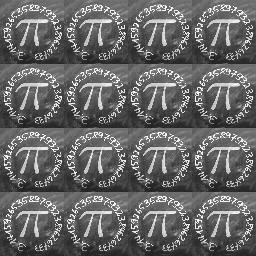
\includegraphics[scale=\myscale,scale=0.3]{images_chapter/pi_gimp_new_photo_2.png}\qquad
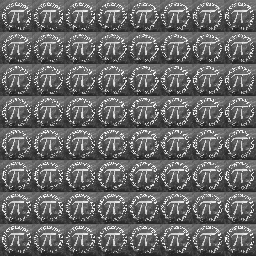
\includegraphics[scale=\myscale,scale=0.3]{images_chapter/pi_gimp_new_photo_3.png}\qquad
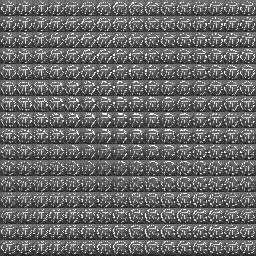
\includegraphics[scale=\myscale,scale=0.3]{images_chapter/pi_gimp_new_photo_4.png}
\end{center}
\begin{center}
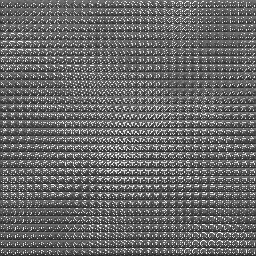
\includegraphics[scale=\myscale,scale=0.3]{images_chapter/pi_gimp_new_photo_5.png}\qquad
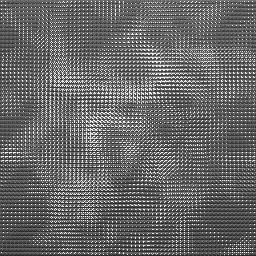
\includegraphics[scale=\myscale,scale=0.3]{images_chapter/pi_gimp_new_photo_6.png}\qquad
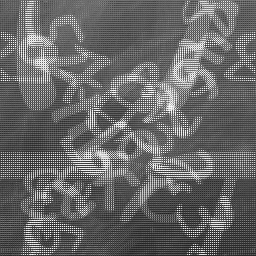
\includegraphics[scale=\myscale,scale=0.3]{images_chapter/pi_gimp_new_photo_7.png}\qquad
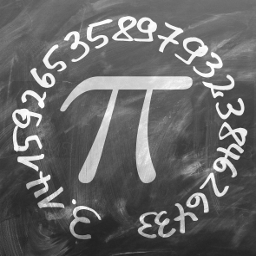
\includegraphics[scale=\myscale,scale=0.3]{images_chapter/pi_gimp_new_photo_8.png}
\end{center}
The image becomes more and more blurred, but after some number transformation, we fall back to the original image!
\end{cours}




%%%%%%%%%%%%%%%%%%%%%%%%%%%%%%%%%%%%%%%%%%%%%%%%%%%%%%%%%%%%%%%%
% Activity 1 - Photomaton transformation
%%%%%%%%%%%%%%%%%%%%%%%%%%%%%%%%%%%%%%%%%%%%%%%%%%%%%%%%%%%%%%%%


\begin{activite}[Photo booth transformation]

\objectifs{Goal: program the photo booth transformation that decomposes an image into sub-pictures. When this transformation is iterated, the image gradually disintegrates, then suddenly re-formes.}



\begin{enumerate}
  \item Program a \ci{transformation(i,j,n)} function that uses the photo booth transformation formula and returns the new coordinates $(i',j')$ of the pixel  $(i,j)$, in the image.
  
  For example, \ci{transformation(1,1,8)} returns \ci{(4,4)}.
  
  \item Program a \ci{photo_booth(array)} function that returns the table calculated by completing a transformation.

For example, the array on the left is transformed into the array on the right.
$$\begin{array}{cccc} 
  1& 2& 3& 4\\ 
  5& 6& 7& 8\\  
  9&10&11&12\\  
 13&14&15&16  
\end{array}\qquad\qquad
\begin{array}{cccc} 
  1& 3& 2& 4\\  
  9&11&10&12\\  
  5& 7& 6& 8\\  
 13&15&14&16
\end{array}$$

  \emph{Hints.} You can initialize a new table with the command:  
  \mycenterline{\ci{new_array = [[0 for j in range(n)] for i in range(n)]}}
  
  Then fill it with commands of the type: 
  \mycenterline{\ci{new_array[ii][jj] = array[i][j]}}

  \item Program a \ci{photo_booth_iterate(array,k)} function that returns the table calculated after $k$ iterations of the photo booth transformation.
  
  \item \emph{To be finished after completing activity 2.}
  
  Program a \ci{photo_booth_images(image_name,kmax)} function that calculates the images corresponding to the transformation, for all iterations from $k=1$ to $k=k_{\max}$.
  
  \item Experiment for different values of the size $n$, to see after how many iterations we return to the original image.
  
\end{enumerate}

Here is the starting image of size $256 \times 256$ and the images obtained by iterations of the photo booth transformation for $k=1$ up to $k=8$. After $8$ iterations we return to the initial image again.
\begin{center}
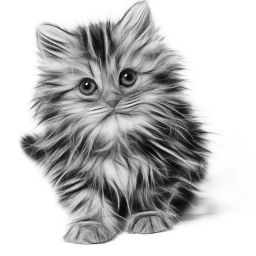
\includegraphics[scale=\myscale,scale=0.4]{images_chapter/cat_gimp_new_photo_0.png}
\end{center}
\begin{center}
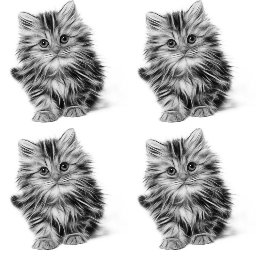
\includegraphics[scale=\myscale,scale=0.3]{images_chapter/cat_gimp_new_photo_1.png}\qquad
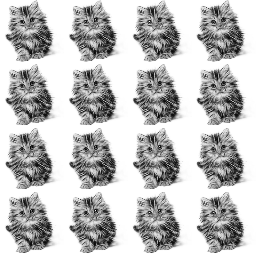
\includegraphics[scale=\myscale,scale=0.3]{images_chapter/cat_gimp_new_photo_2.png}\qquad
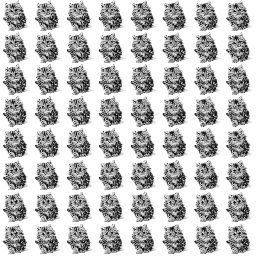
\includegraphics[scale=\myscale,scale=0.3]{images_chapter/cat_gimp_new_photo_3.png}\qquad
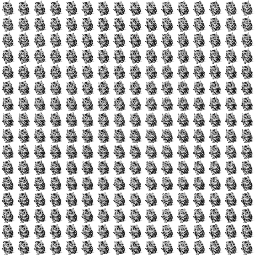
\includegraphics[scale=\myscale,scale=0.3]{images_chapter/cat_gimp_new_photo_4.png}
\end{center}
\begin{center}
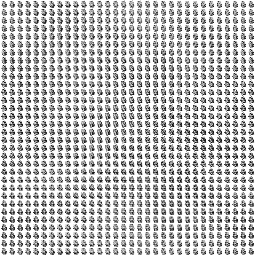
\includegraphics[scale=\myscale,scale=0.3]{images_chapter/cat_gimp_new_photo_5.png}\qquad
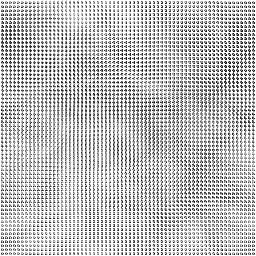
\includegraphics[scale=\myscale,scale=0.3]{images_chapter/cat_gimp_new_photo_6.png}\qquad
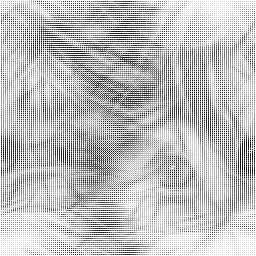
\includegraphics[scale=\myscale,scale=0.3]{images_chapter/cat_gimp_new_photo_7.png}\qquad
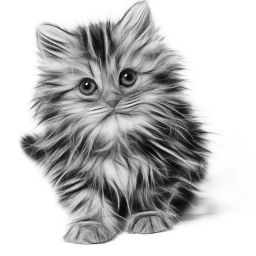
\includegraphics[scale=\myscale,scale=0.3]{images_chapter/cat_gimp_new_photo_8.png}
\end{center}


\end{activite}


%%%%%%%%%%%%%%%%%%%%%%%%%%%%%%%%%%%%%%%%%%%%%%%%%%%%%%%%%%%%%%%%
% Activity 2 - Conversion of table/image
%%%%%%%%%%%%%%%%%%%%%%%%%%%%%%%%%%%%%%%%%%%%%%%%%%%%%%%%%%%%%%%%


\begin{activite}[Conversion array/image]

\objectifs{Goal: switch from an array to an image file and vice versa. The image is displayed in the \og{}pgm\fg{} format which has been manipulated in the \og{}Files\fg{} chapter.}

\index{pbm@\emph{pbm/pgm/ppm}}

\begin{enumerate}
  \item \textbf{Array to image.}
  
  Program an \ci{array_to_image(array,image_name)} function that writes an image  from a grayscale table to a file in \og{}pgm\fg{} format.
  
\begin{center}
\begin{minipage}{0.3\textwidth}
\begin{lstlisting}
P2
5 5
255
128 192 128 192 128
224   0 228   0 224
228 228 228 228 228 
224  64  64  64 224 
192 192 192 192 192 
\end{lstlisting}
\end{minipage}
\begin{minipage}{0.3\textwidth}
\begin{center}

\includegraphics[scale=\myscale,scale=0.15]{input/ecran-test-pgm}
\end{center}
\end{minipage}
\end{center}
For example, with \ci{array = [ [128,192,128,192,128], [224,...] ]}, the \ci{array_to_image(array,"test")} command writes a \ci{test.pgm} file (on the left) to be displayed as the image on the right.

  
  
  \item \textbf{Image to array.} 
  
  Program a \ci{image_to_array(image_name)} function 
  which takes an image file in \og{}pgm\fg{} format and returns an array of gray levels.
\end{enumerate}

\end{activite}


%%%%%%%%%%%%%%%%%%%%%%%%%%%%%%%%%%%%%%%%%%%%%%%%%%%%%%%%%%%%%%%%
%%%%%%%%%%%%%%%%%%%%%%%%%%%%%%%%%%%%%%%%%%%%%%%%%%%%%%%%%%%%%%%%
\begin{cours}[Baker's transformation]

We start from an $n\times n$ array, with even $n$, where each element represents a pixel. We will apply two elementary transformations each time:

\begin{itemize}
  \item \textbf{Stretching.} The principle is as follows: the first two lines (each with a length of $n$) produce a single line with a length of $2n$. We mix the values of each line by alternating an upper element and a lower element.

\medskip
 
\myfigure{1}{
\tikzinput{fig-images-2}
}

Here is how two lines mix into one:
\myfigure{1}{
\tikzinput{fig-images-2bis}
}  

\medskip

\emph{Formulas.} An element at position $(i,j)$ of the target array, corresponds to an element $(2i,j//2)$ (if $j$ is even) or $(2i+1,j//2)$ (if $j$ is odd) of the source array, with here $0 \le i < \frac n2$ and $0 \le j < 2n$.

\medskip

\emph{Example.} Here is a $4 \times 4$ array, and the stretched $2 \times 8$ array.
The rows $0$ and $1$ on the left give the row $0$ on the right.
The rows $2$ and $3$ on the left give the row $1$ on the right.
$$\begin{array}{cccc} 
  1& 2& 3& 4\\ 
  5& 6& 7& 8\\  
  9&10&11&12\\  
 13&14&15&16  
\end{array}\qquad\qquad 
\begin{array}{cccccccc} 
  1& 5& 2& 6& 3& 7& 4& 8  \\
  9&13&10&14&11&15&12&16
\end{array}$$
  
  \item \textbf{Fold.} The principle is as follows: the right part of a stretched array is turned upside down, then added under the left part. Starting from a $\frac n2 \times 2n$ array you get a $n \times n$ array.

 
\myfigure{0.7}{
\tikzinput{fig-images-3}
}  

\emph{Formulas.} 
For $0 \le i < \frac n2$ and $0 \le j < n$ the elements in position $(i,j)$ of the array are kept in place.
For $\frac n2 \le i < n$ and $0 \le j < n$ an element of the array 
$(i,j)$, corresponds to an element $\big(\frac{n}{2} - i - 1,2n-1-j\big)$ of the source array. 


\emph{Example.} 
From the stretched $2 \times 8$ array on the left, we obtain a folded $4 \times 4$ array on the right. 
$$ 
\begin{array}{cccccccc} 
  1& 5& 2& 6& 3& 7& 4& 8  \\
  9&13&10&14&11&15&12&16
\end{array}\qquad\qquad
\begin{array}{cccc} 
  1& 5& 2& 6\\ 
  9& 13& 10& 14\\  
  16&12&15&11\\  
  8&4&7&3  
\end{array}$$
\end{itemize}


The \defi{baker transformation} is the succession of stretching and folding, starting and ending with an $n \times n$ array.


Let's see an example of several baker transformations.
On the left is the initial $128 \times 128$ image, then the result of $k=1,2,3$ iterations. 

\begin{center}
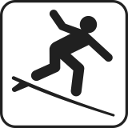
\includegraphics[scale=\myscale,scale=0.65]{images_chapter/surf_gimp_new_baker_0.png}\qquad
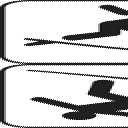
\includegraphics[scale=\myscale,scale=0.65]{images_chapter/surf_gimp_new_baker_1.png}\qquad
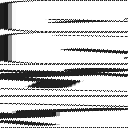
\includegraphics[scale=\myscale,scale=0.65]{images_chapter/surf_gimp_new_baker_2.png}\qquad
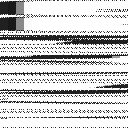
\includegraphics[scale=\myscale,scale=0.65]{images_chapter/surf_gimp_new_baker_3.png}
\end{center}


Here are the images for $k=12,13,14,15$ iterations:

\begin{center}
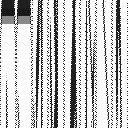
\includegraphics[scale=\myscale,scale=0.65]{images_chapter/surf_gimp_new_baker_12.png}\qquad
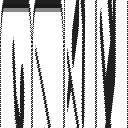
\includegraphics[scale=\myscale,scale=0.65]{images_chapter/surf_gimp_new_baker_13.png}\qquad
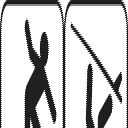
\includegraphics[scale=\myscale,scale=0.65]{images_chapter/surf_gimp_new_baker_14.png}\qquad
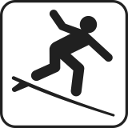
\includegraphics[scale=\myscale,scale=0.65]{images_chapter/surf_gimp_new_baker_15.png}
\end{center}

\end{cours}

%%%%%%%%%%%%%%%%%%%%%%%%%%%%%%%%%%%%%%%%%%%%%%%%%%%%%%%%%%%%%%%%
% Activity 3 - Baker transformation
%%%%%%%%%%%%%%%%%%%%%%%%%%%%%%%%%%%%%%%%%%%%%%%%%%%%%%%%%%%%%%%%


\begin{activite}[Baker's transformation]

\objectifs{Goal: program a new transformation that stretches and folds an image. Once again, the image becomes more and more distorted but, after a certain number of iterations, we return to the original image again.}


\begin{enumerate}
  \item Program a \ci{baker_stretch(array)} function that returns the new array obtained by \og{}stretching\fg{} the input table.

    \item Program a \ci{baker_fold(array)} function that returns the table obtained by \og{}folding\fg{} the input table.
  
   \item Program a \ci{baker_iterate(array,k)} function that returns the table calculated after $k$ iterations of baker's transformation.
  
  For example, the original $4 \times 4$ table is on the left, its image after a transformation ($k=1$) and its image after a second transformation ($k=2$) are also shown.
  
 $$\begin{array}{cccc} 
  1& 2& 3& 4\\ 
  5& 6& 7& 8\\  
  9&10&11&12\\  
 13&14&15&16  
\end{array}\qquad\qquad  
 \begin{array}{cccc} 
  1& 5& 2& 6\\ 
  9& 13& 10& 14\\  
  16&12&15&11\\  
  8&4&7&3  
\end{array}\qquad\qquad  
 \begin{array}{cccc} 
   1&    9&    5&   13 \\ 
 16&    8&   12&    4\\  
  3&   11&    7&   15\\  
 14&    6&   10&    2
\end{array}
$$ 
  \item Program a  \ci{baker_images(image_name,kmax)} function that calculates the images corresponding to baker's transformation, with iterations ranging from $k=1$ to $k=k_{\max}$.
  
  \item Experiment with different values of the size $n$, to see after how many iterations we get back to the original image. 
  
  \emph{Caution!} It sometimes takes many iterations to get back to the original image. For example when $n=4$, we return to the starting image after $k=5$ iterations; when $n=256$ it takes $k=17$. Conjecture a return value in the case where $n$ is a power of $2$. However, for $n=10$, you need $k = 56\,920$ iterations!
   
  
\end{enumerate}

Here is an example with an image of size $256 \times 256$, first the initial image, then one transformation ($k=1$) and a second iteration ($k=2$).
\begin{center}
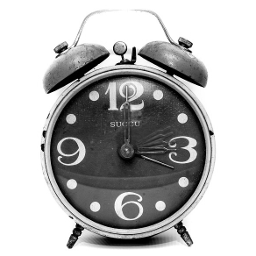
\includegraphics[scale=\myscale,scale=0.4]{images_chapter/clock_gimp_new_baker_0.png}\qquad
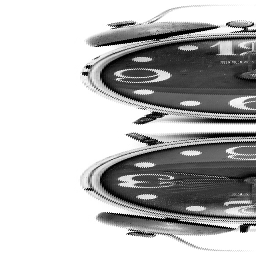
\includegraphics[scale=\myscale,scale=0.4]{images_chapter/clock_gimp_new_baker_1.png}\qquad
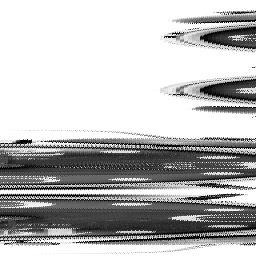
\includegraphics[scale=\myscale,scale=0.4]{images_chapter/clock_gimp_new_baker_2.png}
\end{center}
$k=3,4,5$ :
\begin{center}
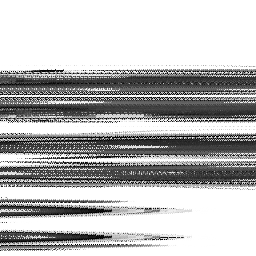
\includegraphics[scale=\myscale,scale=0.4]{images_chapter/clock_gimp_new_baker_3.png}\qquad
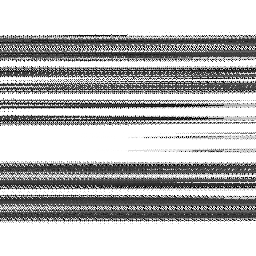
\includegraphics[scale=\myscale,scale=0.4]{images_chapter/clock_gimp_new_baker_4.png}\qquad
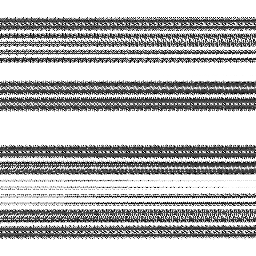
\includegraphics[scale=\myscale,scale=0.4]{images_chapter/clock_gimp_new_baker_5.png}
\end{center}

$k=15,16,17$ :
\begin{center}
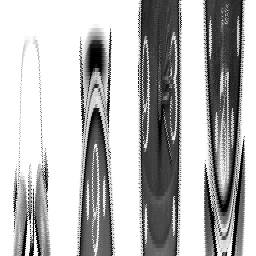
\includegraphics[scale=\myscale,scale=0.4]{images_chapter/clock_gimp_new_baker_15.png}\qquad
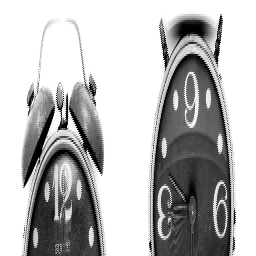
\includegraphics[scale=\myscale,scale=0.4]{images_chapter/clock_gimp_new_baker_16.png}\qquad
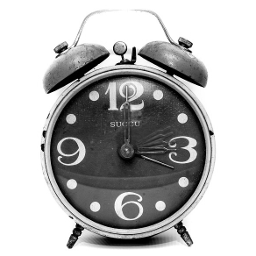
\includegraphics[scale=\myscale,scale=0.4]{images_chapter/clock_gimp_new_baker_17.png}
\end{center}

For $k=17$ you get back to the original image!

\end{activite}


This chapter is based on the article \og{}Blurred images, recovered images\fg{} by Jean-Paul Delahaye and Philippe Mathieu (Pour la Science, 1997).


\end{document}
